\documentclass{beamer}
%
% Choose how your presentation looks.
%
% For more themes, color themes and font themes, see:
% http://deic.uab.es/~iblanes/beamer_gallery/index_by_theme.html
%
\mode<presentation>
{
  \usetheme{default}      % or try Darmstadt, Madrid, Warsaw, ...
  \usecolortheme{default} % or try albatross, beaver, crane, ...
  \usefonttheme{default}  % or try serif, structurebold, ...
  \setbeamertemplate{navigation symbols}{}
  \setbeamertemplate{caption}[numbered]
} 

% My packages
  %  \usefonttheme{default}
  %  \setbeamerfont{title}{series=default,parent=structure}
   % \setbeamerfont{subtitle}{size=\scriptsize,series=\bfseries,parent=structure}
   % \setbeamerfont{author}{size=\scriptsize,series=\bfseries,parent=structure}
   % \setbeamerfont{institute}{size=\scriptsize,series=\bfseries,parent=structure}
   % \setbeamerfont{date}{size=\scriptsize,series=\bfseries,parent=structure}


\usepackage{beamerthemeclassic }

\usepackage{apacite}
\usepackage{natbib}
\usepackage{caption}
\usepackage{amsmath}
\usepackage{graphicx}
\usepackage{adjustbox}
\usepackage{booktabs}
% End my packages


\usepackage[english]{babel}
\usepackage[utf8x]{inputenc}

\title{ML Applications in Marketing:  Optimizing Household Expenditure Predictions}
\author{Charl van Schoor \\ Supervisor: Schahin Tofangchi}
%\institute{Department of Economics, University of Pretoria.}
\date{\today}

\begin{document}

\begin{frame}
  \titlepage
\end{frame}

% Uncomment these lines for an automatically generated outline.
%\begin{frame}{Outline}
%  \tableofcontents
%\end{frame}

\section{The Story}

\subsection{The story}
\begin{frame}{The story}
\begin{block}{Consumer behavior}
\begin{itemize}
  \item Hedonistic versus utilitarian consumption. 
  \item Can we empirically test for, predict and extract information about, hedonistic consumption behaviour using ML.
  \item Utilizing predictive and explanatory statistics. 

%  \item Use \texttt{itemize} to organize your main points.
\end{itemize}
\end{block}
\begin{block}{Literature}
\begin{itemize}

  \item \cite{hirschman1982hedonic}
  \item \cite{shmueli2010explain}
  \item \cite{babin}

%  \item Use \texttt{itemize} to organize your main points.
\end{itemize}
\end{block}
\end{frame}




\begin{frame}{The Story}
\begin{block}{Purpose}
Can we predict whether a consumer is utilitarian or hedonistic? In this case, can we predict whether a consumer will purchase a gift or not? We want to see what factors, or topics, contribute the most to consumer behaviour related to giving. Thus, LDA with Logistic regression. 
\end{block}

\begin{block}{What is the contribution?}
\begin{itemize}
\item Practically: The method can be employed by retailers to model the distribution of individual consumers over specific topics. 
\item Theoretically: Serve as an example between the use of both predictive and explanatory modeling. 
\end{itemize}
\end{block}

\vskip 1cm
\end{frame}



%\begin{frame}[plain]{Some maps}
% Commands to include a figure:
%\begin{figure}
%\includegraphics[width=0.9\textwidth]{graphs/GDP_pc_TFP_growth.png}
%\caption{\label{fig:your-figure}Trade Margins}
%\end{figure}
%Source data: GDPpc optained from USDA, TFP from PWT
%\end{frame}

 
% --------------------------------------------------------------------------------------------------------------------------------




\section{Methodology} % (fold)
\label{sec:the_maths}




\subsection{Methodology and Dataset}
\begin{frame}{Data}
\begin{block}{Data}
\begin{itemize}
\item The dataset is sourced from the \cite{bls} and contains household expenditure data. Put differently, households were asked to keep a diary of frequently purchased items over a period of two weeks. 
\item The dataset includes all purchases over the period and it also includes descriptions of the products purchased. It also contains other variables indicating the demographics of the household and an indicator for whether they bought a gift. 
\end{itemize}
\end{block}
\end{frame}


\begin{frame}{Data}
\begin{block}{Data: The Dimensions}
\begin{itemize}
\item 57195 unique households (NEWID)
\item 548 unique products and descriptions (UCC)
\item Time dimension removed over the period
\end{itemize}
\begin{figure}
\includegraphics[scale=0.4]{/Users/charlvanschoor/Documents/Gottingen/ML/jedi/Final/R/LDA/graphs/newiddata.png}
\caption{\label{fig:your-figure}Basic Data}
\end{figure}
\end{block}
\end{frame}


% \begin{frame}{Data}
% \begin{block}{Data}
% \begin{itemize}
% %include pictures of control variables
% %include pictures of variables (Gift UCC)
% %include pictures of description (Before and after wikipedia)

% \end{itemize}
% \end{block}
% \end{frame}

%\begin{frame}[plain]{Some maps}
% Commands to include a figure:
%\begin{figure}
%\includegraphics[width=0.9\textwidth]{graphs/GDP_pc_TFP_growth.png}
%\caption{\label{fig:your-figure}Trade Margins}
%\end{figure}
%Source data: GDPpc optained from USDA, TFP from PWT
%\end{frame}






\begin{frame}{Methodology}
\begin{block}{Topic model: LDA}
\begin{itemize}
\item The Topic modeling method used is Latent Dirichlet Allocation. 
\item The problem: the descriptions of the products don't contain enough information about the product to model different topics.
\end{itemize}
\begin{figure}
\includegraphics[scale=0.4]{/Users/charlvanschoor/Documents/Gottingen/ML/jedi/Final/R/LDA/graphs/descriptions.png}
\end{figure}
\end{block}
\end{frame}


\begin{frame}{LDA}

\begin{itemize}
\item The solution: Wikipedia 
\end{itemize}

\begin{figure}
\includegraphics[width=0.9\textwidth]{/Users/charlvanschoor/Documents/Gottingen/ML/jedi/Final/R/LDA/graphs/descriptionsWiki.png}
\end{figure}

\end{frame}


\begin{frame}{LDA - The Intuition}

\begin{itemize}
\item The idea is to model each product description into a set of topics. Intuitively, we want each product description to have a value that represents the probability that the given description belongs to a certain topic. 
\item By doing this we can reduce the dimensionality of the data and use it for further analysis. 
\item Each product thus has a probability that it belongs to a certain topic. This means that each product is distributed along the topics, but for some more than others.
\end{itemize}

\end{frame}



\begin{frame}{LDA - Layout}
\begin{figure}
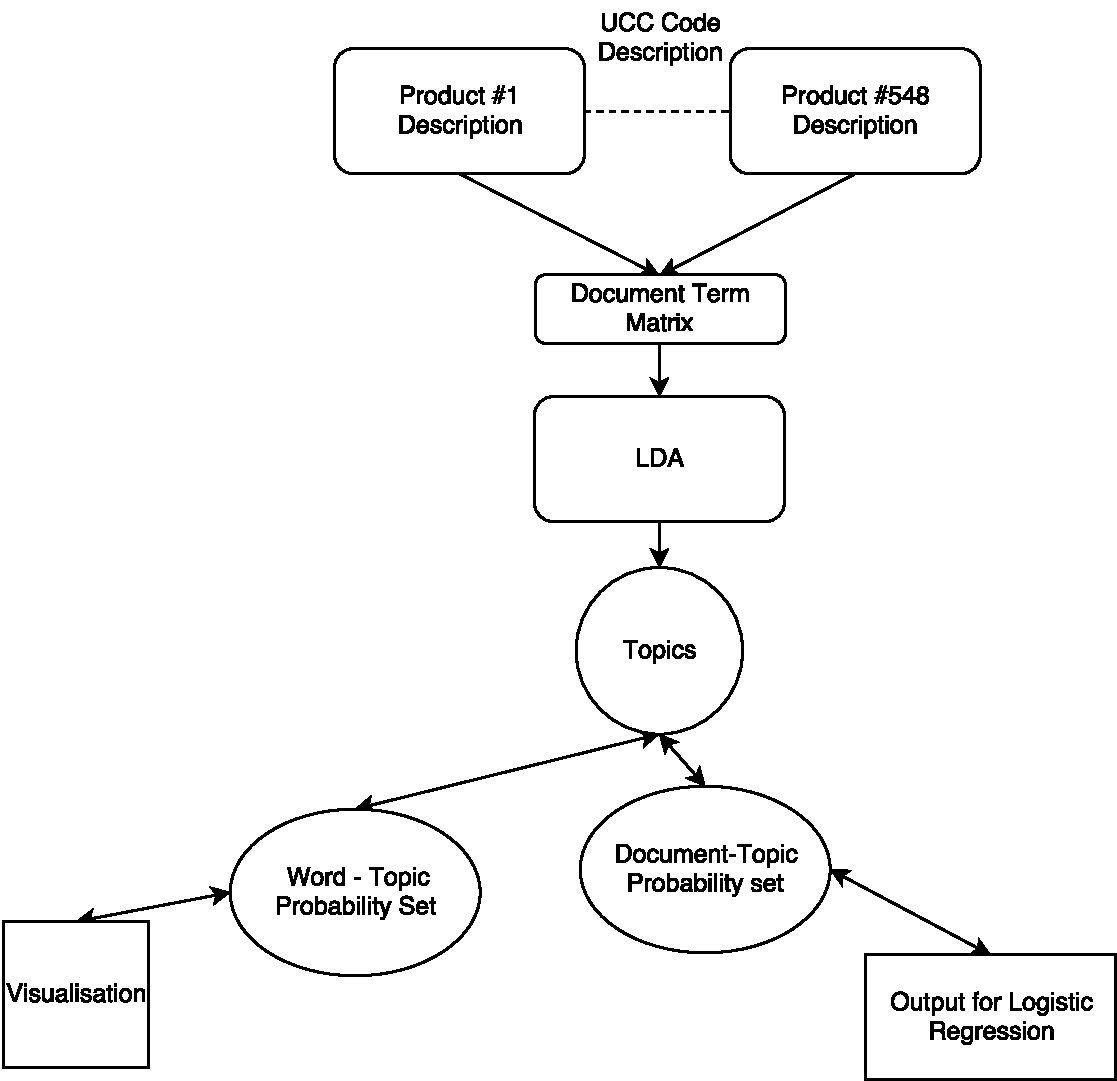
\includegraphics[width=0.65\textwidth]{/Users/charlvanschoor/Documents/Gottingen/ML/jedi/Final/R/LDA/graphs/LDA.pdf}
\end{figure}
\end{frame}



\begin{frame}{LDA - Some Figures}

\begin{figure}
\includegraphics[width=1\textwidth]{/Users/charlvanschoor/Documents/Gottingen/ML/jedi/Final/R/LDA/graphs/wordCountperCode.pdf}
\end{figure}
\end{frame}

\begin{frame}{LDA - Some Figures}

\begin{figure}
\includegraphics[width=1\textwidth]{/Users/charlvanschoor/Documents/Gottingen/ML/jedi/Final/R/LDA/graphs/distrTopicoverCodetend.pdf}
\end{figure}

\end{frame}

\begin{frame}{LDA - Some Figures}

\begin{figure}
\includegraphics[width=1\textwidth]{/Users/charlvanschoor/Documents/Gottingen/ML/jedi/Final/R/LDA/graphs/UCCdistrTopics.pdf}
\end{figure}

\end{frame}

\begin{frame}{LDA - Some Figures}

\begin{figure}
\includegraphics[width=0.65\textwidth]{/Users/charlvanschoor/Documents/Gottingen/ML/jedi/Final/R/LDA/graphs/topicsper10.pdf}
\end{figure}

\end{frame}







\begin{frame}{Methodology}
\begin{block}{Logistic Regressions: Topic Data}
\begin{itemize}
\item We now have the topics and the probability of each product belonging to a topic. But we want to model the households over the topics (i.e. get a distribution of the topics representing each household)
\item I do this by multiplying the probability of each product, given the topic, with the amount of times the household bought each product. 
\item Thereafter I normalize the topics for each household by taking the unit root of all the products. 
\item Thus, a distribution for each household over each topic. 
\end{itemize}
\end{block}
\end{frame}

\begin{frame}{Logistic Regressions: Topic Data in Math}


\[Topi{c_i}(k) = \frac{{\sum\limits_{j = 1}^{548} {({\gamma _j}(k)*{n_{ij}})} }}{{\sqrt {\sum\limits_{k = 1}^K {{{\left( {\sum\limits_{j = 1}^{548} {({\gamma _j}(k)*{n_{ij}})} } \right)}^2}} } }}\]

\

where \textit{i} is each individual household, \textit{j} is each individual product and \textit{k} is each individual topic. The \textit{n} represents the amount of times a consumer purchased a particular product. 

\end{frame}



\begin{frame}{Logistic Regressions}
\begin{block}{First Level}

\[Gift{_i} = Topic{_i}(1) + ... + Topic{_i}(K)\]
\end{block}

\begin{block}{Second Level}

\[Gift{_i} = Topic{_i}(1) + ... + Topic{_i}(K) + Inc{_i} + Educ{_i} + Sex{_i} + Age{_i} + \sum\limits_{s = 1}^{55} {State{_{si}}} \]
\end{block}
\end{frame}










% --------------------------------------------------------------------------------------------------------------------------------



\section{Results} 
\begin{frame}{Results}

\begin{block}{GLM: Topics}
\begin{figure}
\includegraphics[width=0.65\textwidth]{/Users/charlvanschoor/Documents/Gottingen/ML/jedi/Final/R/LDA/graphs/topicshed.png}
\end{figure}
\end{block}

\end{frame}


\begin{frame}{Results}

\begin{block}{GLM: Topics}
\begin{figure}
\includegraphics[width=0.65\textwidth]{/Users/charlvanschoor/Documents/Gottingen/ML/jedi/Final/R/LDA/graphs/topicsutil.png}
\end{figure}
\end{block}

\end{frame}


\begin{frame}{Results}

\begin{block}{GLM: All Predictors}
\begin{figure}
\includegraphics[width=0.65\textwidth]{/Users/charlvanschoor/Documents/Gottingen/ML/jedi/Final/R/LDA/graphs/allhed.png}
\end{figure}
\end{block}

\end{frame}


\begin{frame}{Results}

\begin{block}{GLM: All Predictors}
\begin{figure}
\includegraphics[width=0.65\textwidth]{/Users/charlvanschoor/Documents/Gottingen/ML/jedi/Final/R/LDA/graphs/allutil.png}
\end{figure}
\end{block}

\end{frame}

\begin{frame}{Results}

\begin{block}{GLM: Confusion Matrix}
\begin{figure}
\includegraphics[width=0.65\textwidth]{/Users/charlvanschoor/Documents/Gottingen/ML/jedi/Final/R/LDA/graphs/confumat.png}
\end{figure}
\end{block}

\end{frame}
% --------------------------------------------------------------------------------------------------------------------------------


\begin{frame}{In other words..}
\begin{itemize}
  \item Using topic modeling seems to be an interesting approach to reduce the dimensionality of the data. However, the results are subject to the amount of topics specified. 
  \pause{} 
  \item Moreover, the predictive capability of the GLM does not seem to fit the data. Another method should be used for prediction. 
  \pause{} 
  \item GLM does offer some explanatory power. The top hedonic predictors contained descriptions like: Tires, wear, coal, oil, vehicle etc.. Another top predictor is a male dominated household.
  \pause{} 
  \item The top utilitarian predictors contained descriptions like: Pub, culture, clocks, decorative, public, transport etc. Another top predictor is a high level of education within the household. 
\end{itemize}

\end{frame}

\begin{frame}{Still to come}
\begin{itemize}
  \item NN for prediction
  \item Different dependent variables
  \item More or less topics
\end{itemize}

\end{frame}
% subsection expected_results_and_possible_limitation (end)

% subsection references (end)
% section references (end)
\subsection{Discussion} % (fold)
\label{sub:discussion}
\section{Discussion} % (fold)
\label{sec:discussion}

% section discussion (end)
% subsection discussion (end)
\begin{frame}{Discussion}



\end{frame}
\begin{frame}{Bibliography}
	\bibliography{bib}\newpage
	\bibliographystyle{apacite} \newpage
\end{frame}
\end{document}